\documentclass[11pt]{article}

\usepackage[utf8]{inputenc}
\usepackage[english]{babel}

\usepackage{mathtools}

\usepackage{setspace}
\onehalfspacing

\usepackage{amsfonts}
\usepackage{amsmath}
\usepackage{amsthm}
\usepackage{indentfirst}
\newtheorem{theorem}{Theorem}
\newtheorem{lemma}{Lemma}
\newtheorem{example}{Example}
\newtheorem{definition}{Definition}
\newtheorem{remark}{Remark}
\newtheorem{corollary}{Corollary}

\newtheorem*{theorem*}{Theorem}
\newtheorem*{lemma*}{Lemma}
\newtheorem*{example*}{Example}
\newtheorem*{definition*}{Definition}
\newtheorem*{remark*}{Remark}
\newtheorem*{corollary*}{Corollary}

%\usepackage{booktabs, caption, graphicx, float}
%\usepackage{subcaption}
%\captionsetup{tableposition=top,figureposition=bottom,font=small}

\usepackage{comment}
\usepackage{multirow}
\usepackage{array}

\newcolumntype{C}[1]{>{\centering\let\newline\\\arraybackslash\hspace{0pt}}m{#1}}
\DeclarePairedDelimiter\floor{\lfloor}{\rfloor}

\usepackage[hidelinks]{hyperref}

\usepackage{geometry}
\geometry{a4paper, top=3cm,bottom=3cm,left=3cm,right=3cm,%
	heightrounded}
\usepackage{upgreek}
\usepackage{xparse}
\usepackage{listings}
\NewDocumentCommand{\codeword}{v}{%
	\texttt{\textcolor{black}{#1}}%
}

\newcommand{\prepos}[3]{${}_{\mathbf{#2}}{\mathbf{#1}}_{#3}$}
\newcommand{\preposm}[3]{{}_{\mathbf{#2}}{\mathbf{#1}}_{#3}}


%Dummy text
\usepackage{lipsum}

%Changing headers and footers
\usepackage{fancyhdr}
\pagestyle{fancy}
\fancyhf{}
\rhead{\textit{\thepage}}
\lhead{\textit{ LAB 8: Admittance Control and Planning}}

%For inserting the code
\usepackage{fancyvrb}

%For bold math symbols
\usepackage{bm}

%For multicolumns
\usepackage{multicol}

% Norm and abs delimiter
\usepackage{mathtools}
\DeclarePairedDelimiter{\abs}{\lvert}{\rvert}
\DeclarePairedDelimiterX{\norm}[1]{\lVert}{\rVert}{#1}

\setcounter{section}{-1}

% Argmin/Argmax
\DeclareMathOperator*{\argmax}{argmax}
\DeclareMathOperator*{\argmin}{argmin}

% Enumerate
\usepackage{enumitem}

% Code
\usepackage{algorithm}
\usepackage[noend]{algpseudocode}
\usepackage{etoolbox}

% Longtable
\usepackage{longtable}

% SI units
\usepackage{siunitx}
\sisetup{output-exponent-marker=\ensuremath{\mathrm{e}}}

% Colours in equations
\usepackage{xcolor}

\newcommand{\Rnum}{\mathbb{R}} % Symbol fo the real numbers set
\newcommand{\mat}[1]{\ensuremath{\begin{bmatrix}#1\end{bmatrix}}}	% matrix
\newcommand{\myparagraph}[1]{\paragraph{#1}\mbox{}\\}


\title{LAB 8: Admittance Control and Planning}
\author{Michele Focchi and Matteo Saveriano}
\date{}

\begin{document}
	\maketitle
	\noindent
	The goals of this assignment are:
	\begin{itemize}
		\item learning the basic procedure to design an admittance controller for the end-effector of a manipulator in contact with the environment with the purpose to control the interaction with a human.
		\item Implement an obstacle avoidance planning algorithm base on potential fields. 
	\end{itemize}
	
	\noindent
	Tools that we are going to be using in this lab (all open-source):
	\begin{itemize}
				\item Python programming (2.7/3.5)\footnote{https://docs.python.org/}
				\item Robot Operating System (ROS)\footnote{https://www.ros.org/}
						\item Gazebo \footnote{http://gazebosim.org/}
										\item Pinocchio Library for Rigid Body Dynamics Algorithms\footnote{https://github.com/stack-of-tasks/pinocchio}
				\item Locosim\footnote{https://github.com/mfocchi/locosim}
	\end{itemize}
	%
	%
	%\noindent
	In this assignment we will modify the set-point for the end-effector computed in previous labs, using an admittance model, to accommodate for an external force acting at the end-effector. An inverse kinematics scheme will map the new references into joint references. We will close the loop for tracking at the joint level. The implementation of and admittance control scheme is the only way to be able to  achieve safe interactions with industrial robots that accept only position (and not torque) references. Indeed, most of the times, industrial robots are not equipped with an inner torque loop, but with a (stiff) position loop at the low level, plus a 6 axis force sensor located at the end-effector. Differently from the approaches seen until now, that enable a safe interaction with any part of the robot, this approach allows the robot to be compliant (and safe) \textit{only} if the interaction occurs at the end-effector location, where we are able to \textit{sense} the force. 
	
\section{Preliminaries}
	The robot that we will use this time, is the  6DoFs Ur5 robot (see Fig. \ref{fig:ur5_robot_kinematics}), but, differently from before, we will not integrate the dynamics by ourself with a forward Euler method,  but this task will be delegated to a simulator called Gazebo. An intermediate controller ( \codeword{ros_impedance_controller}) will receive the PD gains and the set-points (of desired joint positions and velocities) and feed-forwards for the torques generated by our Python node.
	The  \codeword{ros_impedance_controller} will either interface to the  Gazebo simulator or to the real robot. This has the big advantage of  allowing us to use the \textit{same} code in both situations, and safely test our algorithm before going on the real robot.\\
	
	
	For this part of the assignment, we will use these four main files: 
	\begin{itemize}
		\item \codeword{LOCOSIM/robot_control/base_controllers/base_controller_fixed.py} (Mother class with a generic controller for fixed based manipulators)
		\item \codeword{LOCOSIM/robot_control/base_controllers/L8_admittance.py} (Main file to run the visualization and all exercises (inherits from BaseControllerFixed))
		\item \codeword{LOCOSIM/robot_control/params.py} (Initializations of variables and simulation parameter for UR5)
		\item \codeword{LOCOSIM/robot_control/L8_conf.py} (Initializations of variables specific for L8 lab exercises)
        \item \codeword{LOCOSIM/robot_control/base_controllers/obstacle_avoidance/obstacle_avoidance.py} (Class that implements the artificial potential field planner)
        \item \codeword{LOCOSIM/robot_control/base_controllers/admittance_controller.py} (Class that implements the admittance model and controller)
        \item \codeword{LOCOSIM/robot_control/base_controllers/components/inverse_kinematics/inv_kinematics_pinocchio.py} (Class that implements numerical inverse kinematics for a generic fixed based robot based on Pinoccchio library)
	\end{itemize}
	
	\begin{figure}[bht]
		\centering
		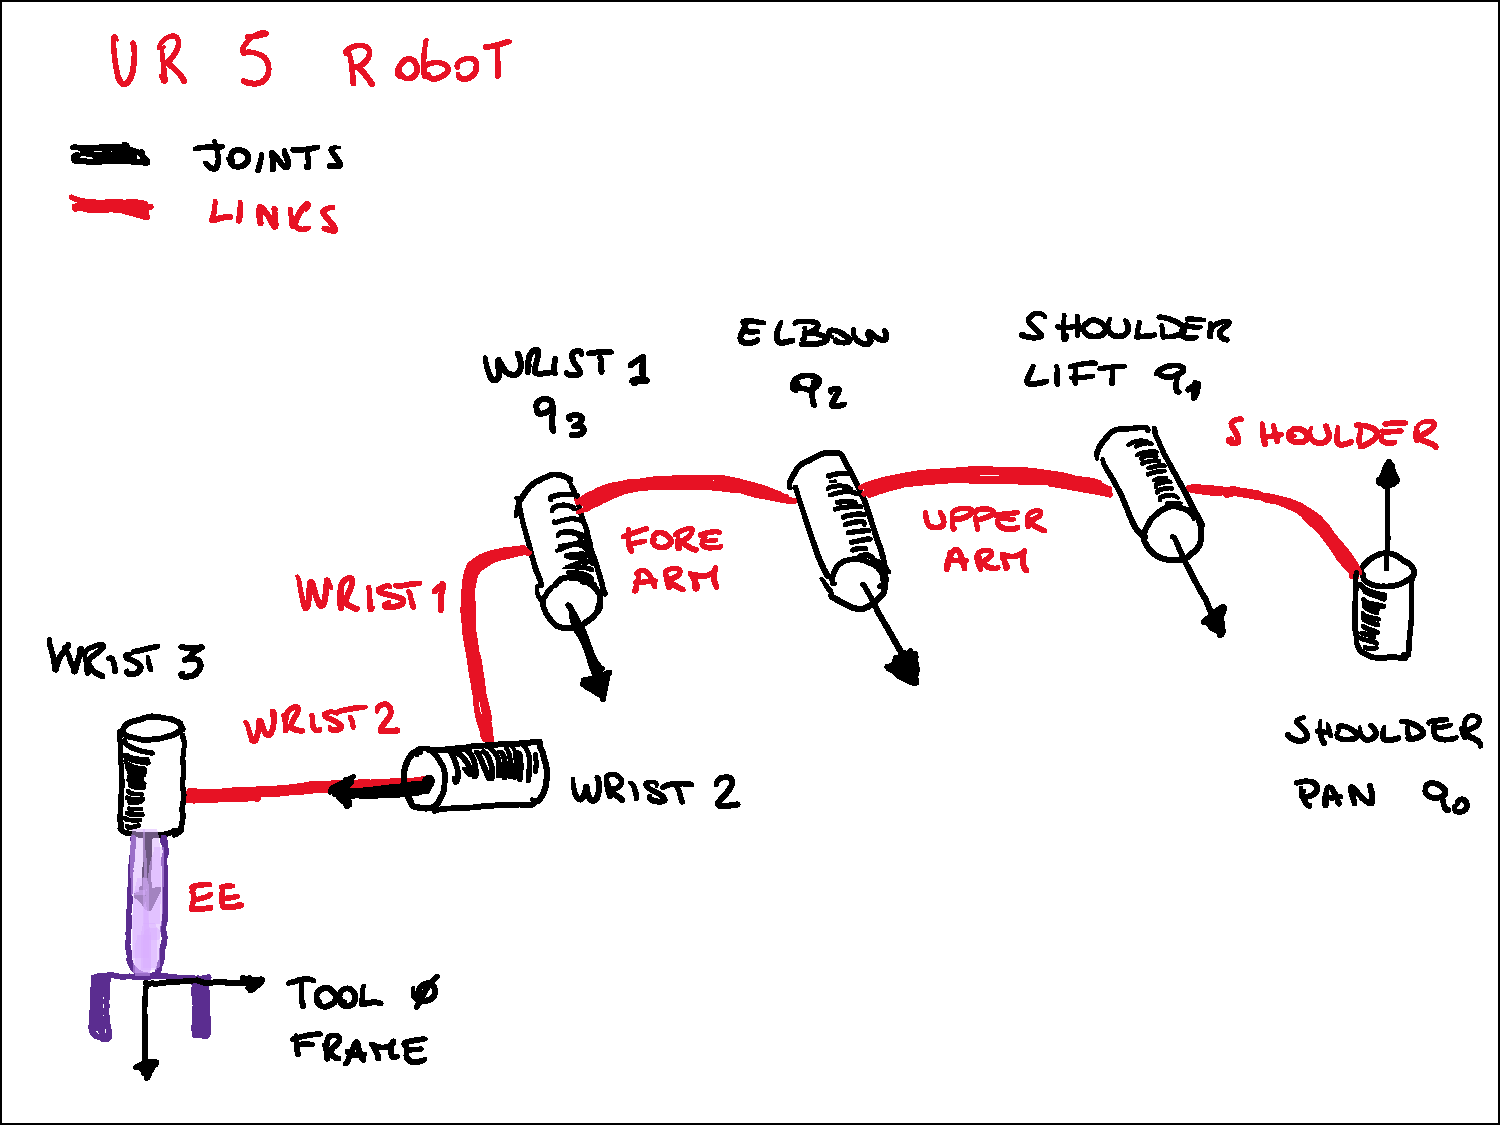
\includegraphics[width=10cm]{pics/ur5_Robot.pdf}
		\caption{Sketch of the UR5 robot kinematics}
		\label{fig:ur5_robot_kinematics}
	\end{figure} 

\section{Position Control}

\textbf{1.1 Position Control - Constant Joint Reference}\\
Since the real prototype of the UR5 robot it does not accept desired torque command but only position and velocity commands, 
the first experience we are going to do is to create a constant set-point in position for our robot. 
Therefore, in the \codeword{params.yaml} configuration file, set \codeword{real_robot: True},   
\codeword{control_mode: point}, \codeword{control_type: position}.
Then, to check that everything works, set a constant reference for joint position equal $q^0=\mat{ 0.5& -1.0& 1.0& -1.7& -1.7& 0.0}^T$.
Note that the real robot might start in a different configuration and to avoid abrupt motions you need to implement a \textit{homing} procedure to drive smoothly the joints to  the  $q^0$ set-point. \\

\textbf{1.2 Position Control - Sinusoidal  Joint Reference.}\\
Now set a sinusoidal reference starting from the  $q^0$ configuration with amplitude $A= 0.15$ $rad$ and frequency $f = 0.25$ $Hz$ equal for all the joints.

\begin{align*}
q^d(t) = q_0 + Asin(2\pi f t )
\end{align*} 

 Try to avoid to set too large amplitude in order to avoid hitting some obstacles. 
 Now that we are using Gazebo as a simulator you can set the fields \codeword{ <dynamics damping="0.0" friction="0.0"/>} in the joint's tag to emulate the effect of viscous friction (damping parameter) and static friction (friction parameter) at the joint. Observe the effect of friction in the tracking of a sinuoidal trajectory as we did for the DC motor.
 \\

\textbf{1.3 Position Control - Constant Cartesian Reference}\\
Now let's set a constant Cartesian position (expressed in the base frame, check the base frame axes) 
for the end-effector $p_e^d=\mat{-0.3&  0.5& -0.5}^T   $. Employ the inverse kinematics function implemented in L1-2.6 and solve the redundancy  setting a postural task $q^p = q_0$.\\

\textbf{1.4 Position Control - Constant Cartesian Reference and Orientation.}\\
In addition to the end-effector position, now we want also to specify a desired orientation with ${}_WR_e^d = eul2rot(\mat{-1.9& -0.5& -0.1})$.
In this case the task is 6D and there is no need of regularization or of a postural task, because the full Jacobian $J6 \in \Rnum^{6 \times 6}$ should we used. 
Note that the now we have to append also  the orientation error $e_o$  to $e_p$. This can be computed with the angle-axis approach or equivalent way as we did for the L3 lab: 

\begin{align}
e_o = \text{logm}({}_wR_e^T {}_wR_e^d)
\end{align}


\textbf{1.5 Position Control - Polynomial trajectory}\\
If you implemented both 1.2 and 1.3 on the real robot, you will notice that the robot goes into protection mode because we are setting an abrupt change in the position set-point $q^d$ that goes from $q_0$ to $IK(p_e^d)$.
Taking inspiration from L1-2.5, design polynomial  trajectories (if you want you can create a class for this) for the end-effector Cartesian coordinates to go from the actual position ($FK(q^0)$) to $p_e^d$. You can start with a quintic polynomial and set zero initial /final velocity and accelerations. Note that only for the quintic it will be possible to enforce the accelerations. Do the implementation also for a cubic polynomial and compare the results. We leave as an exercise the creation of polynomials also for the orientation (hint. use Euler Angles).\\


\section{Admittance Control}
An admittance control framework requires two components: an \textit{admittance model} and an \textit{inverse kinematics} function.
The philosophy behind \textit{admittance} control is to change the end-effector position set-point in order to mimic a desired admittance at the end-effector. 
\footnote{Mechanical admittance is the reciprocal of impedance} We recall that an admittance is a linear model that receives  as input a \textit{force} and 
outputs a displacement $\Delta p_e$ (or a velocity). Then, the displacement $\Delta p_e$ is added to the set-point creating a new reference for the end-effector $\tilde{p_e}^d = \Delta p_e + {p_e}^d$  This can be mapped to joints references via an inverse kinematics function, as shown in figure \ref{fig:admittance}, or we can directly map $\Delta p_e$ via a jacobian to joint displacements $\Delta{q}$ and then sum them to $q^d$:\\

\begin{figure}[bht]
	\centering
	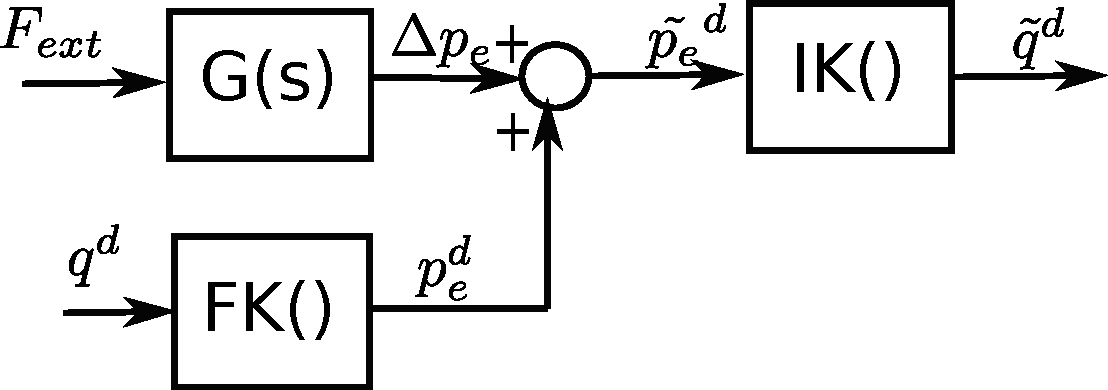
\includegraphics[width=8cm]{pics/admittanceControl.pdf}
	\caption{Block diagram for an admittance controller in the Cartesian space. FK(.) and IK(.) are the forward (or direct) and inverse kinematics blocks, respectively, while G(s) is the admittance model.}
	\label{fig:admittance}
\end{figure}

\textbf{2.1 - Implement the admittance model }\\
We want to implement an admittance model that represents a \textit{linear} virtual spring and a \textit{linear} virtual damper at the end-effector.
The transfer function G(s) for this model in the Laplace domain is :



\begin{align}
\label{eq:tf}
\Delta p_e &= \frac{ F_{ext} }{D_x s + K_x}\\
G(s)& = \frac{\Delta p_e}{F_{ext}} = \frac{ 1 }{D_x s + K_x} \nonumber
\end{align}


Where the input is the contact force $F_{ext}\in \Rnum^3$ and the output the shift  $\Delta p_e\in \Rnum^3$ to be applied to the end-effector reference to emulate a virtual stiffness in response to  $F_{ext}$. Note that this transfer function is in continuous time and we need a discretized version for a digital implementation on a computer. To get the discrete version, it is convenient to convert \eqref{eq:tf} first in the time domain:

\begin{align*}
D_x \Delta\dot{ p_e} + K_x{\Delta p_e}  =  F_{ext}  
\end{align*}
 
Then, if  we  employ Backward Differentiation Formula $\dot{p_e} = (p_e(k)- p_e(k-1))dT^{-1}$ to approximate the derivative, then we can get the following difference equation:

\begin{align*}
&D_x \frac{\Delta p_e(k)- \Delta p_e(k-1)}{dT}  + K_x \Delta p_e(k)  =  F_{ext}(k)  \\
&\Delta p_e(k) (D_x dT^{-1} + K_x ) - D_x \Delta p_e(k-1)dT^{-1} =  F_{ext}(k)\\
&\Delta p_e(k) =  (D_x dT^{-1} + K_x )^{-1} (F_{ext}(k) + D_x \Delta p_e(k-1)dT^{-1})
\end{align*}

where (k)and (k-1) refer to the actual and previous samples of the variables. \\

\textbf{2.2 Inverse Kinematics}\\
Now that we wrote a function to implement the admittance model, we still miss to implement the inverse kinematics function. To be able to convert the modified reference $\tilde{p_e}^d(k) = p_e^d(k) +  \Delta p_e(k)$  at each loop $k$ into a joint reference $q^d$. Note that, since our admittance model (composed of linear spring and damper)  involves only 3D vectors, and we have 6 DoFs in our robot, we will have redundancy, hence  infinite solutions to the inverse kinematics problem. To solve this we will reuse the postural task implementation described in LAB L1-2.4 setting  $q^p = q_0$.\\


\textbf{2.3 - External push with a constant reference}
Now we are ready to test the implemented algorithm. Set  a constant joint reference $q_0$  for the robot to follow (this will correspond to a constant end-effector position $p^d$ that you will have to compute) and set the admittance gains to $K_x = 1000I_{3\times3}$,  $D_x = 300I_{3\times3}$. We can have a feeling  on how the controller works by applying an external force either in simulation (calling the function \codeword{applyForce()} after 5 seconds) or pushing manually (gently!) the end-effector on the real robot (Important! keep always the E-stop in your hand to kill the robot in case some instability arise!). You should feel the robot deviating from the reference in the same direction of the force (we are setting a diagonal stiffness matrix), as if a spring is attached at the end-effector trying to push it back to the original position. 
Now try to reduce the stiffness gain to $K_x = 600I_{3\times3}$, in order to make the robot more ``soft''. You should feel that for the same force you are applying you are getting a bigger deflection (almost double).
Plot the signals of the end-effector position and force to evaluate the direction of the deflection is consistent with the force.\\

\textbf{2.4 - External push with a sinusoidal reference}
Let's now apply a sinusoidal reference to the robot joints  with amplitude $A= 0.15$ $rad$ and frequency $f = 0.25$ $Hz$, around the initial position $q_0$.
And repeat the previous experiment. You will see the robot will deviate in a compliant way from the prescribed trajectory, allowing safe human-robot interaction.\\



%Now, apply the external disturbance, \textit{while} the robot is moving. You should see the end-effector deviating from the original trajectory in the direction of the pushing force. \\
 
 
\textbf{2.5 - Payload estimation.}\\
The final exercise of this lab will be to estimate a payload attached at the end effector in static conditions. We want to exploit the readings from the  joint torques that are stored in the variable \codeword{tau}. Employing the principle of Virtual works we can estimate the an external force applied at the end-effector via the transpose of the end-effector Jacobian. Note that we will have also joint gravity torques to take into consideration that must be discarded.
The derivation of the formula is the following, we start from the dynamic equation of the robot considering an external force $F$ is applied from the environment, and set the joint accelerations and velocities to zero:

\begin{align*}
g &= \tau  + J^TF \\
F &= -(J^T)^\dagger (\tau - g) 
\end{align*}

Note that you need to use the pseudo-inverse of the jacobian J to match dimensions.  Then the payload weight is:
\begin{align*}
m_p = -F_z / g 
\end{align*}

Finally, apply some filtering to take out the noise. 




\section{Potential fields for obstacle avoidance}
In this assignment you will be developing code to guide the end-effector of the robot from one location to another in a
3D  Cartesian space using \textit{artificial potential fields}. Figure \ref{fig:pot_fields} depicts 
the energy surface associated with an  environment with 4 obstacles. The end-effector of the robot is modeled by
the red sphere which we can think of as rolling down the energy surface towards the goal location (green).


\begin{figure}[bht]
	\centering
	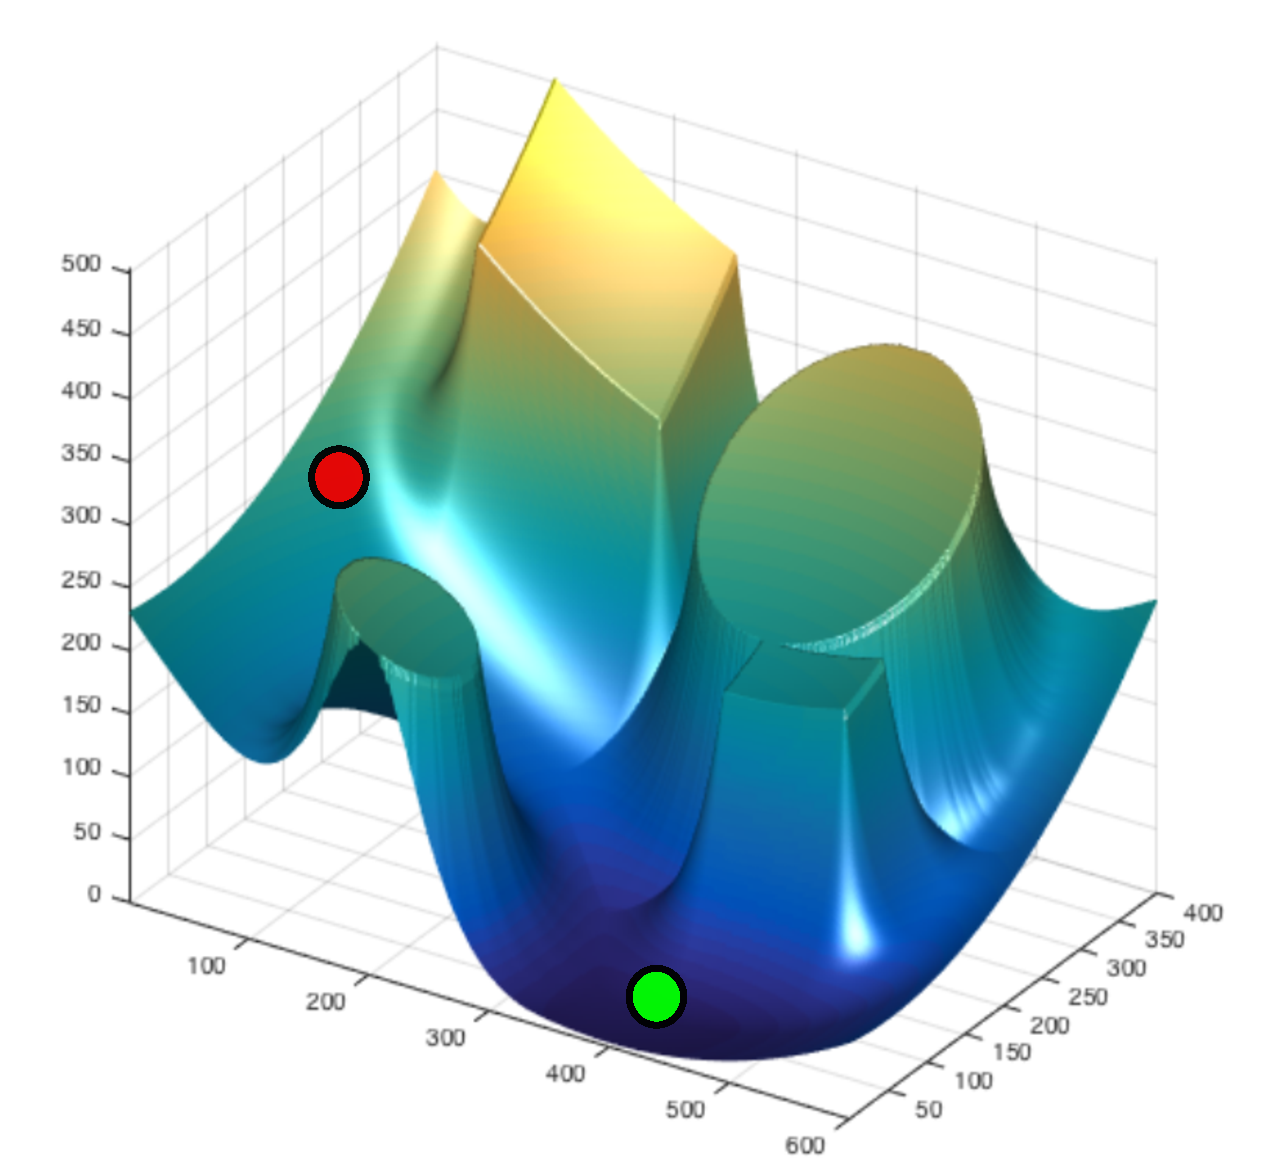
\includegraphics[width=10cm]{pics/pot_fields.pdf}
	\caption{Sketch of an energy surface associated to artificial potential field with a few obstacles, the red ball represents the starting point, the green ball represents the goal.}
	\label{fig:pot_fields}
\end{figure} 

Create a \codeword{GradientBasedPlanner} to control the motion of the robot to arrive to the goal $p_g = \mat{0.7& 1.1& 1.2}^T$.
We want to create an attractive field for the end-effector $p$ to attain the goal $p_g$:

\begin{equation}
f_a(p) = \begin{cases}
k_{a} \mathbf{e}(p)  \quad if \quad  \|\mathbf{e}(p)\| \leq d \\
k_{b} \frac{\mathbf{e}(p)}{\|\mathbf{e}(p)\|}   \quad if \quad  \|\mathbf{e}(p)\| > d \\		
\end{cases}
\end{equation}

where $e = p_g -p$ with $k_{b} = d k_{a}$ to ensure field continuity at $d = 0.2 m$ and field strength $k_a = 8$.
In addition we have  two obstacles in the workspace: one cylinder and a box (see in black in Fig. \ref{fig:workspace}) whose parameters 
are reported in Table  \ref{tab:obstacles}: 

\begin{figure}[H]
	\centering
	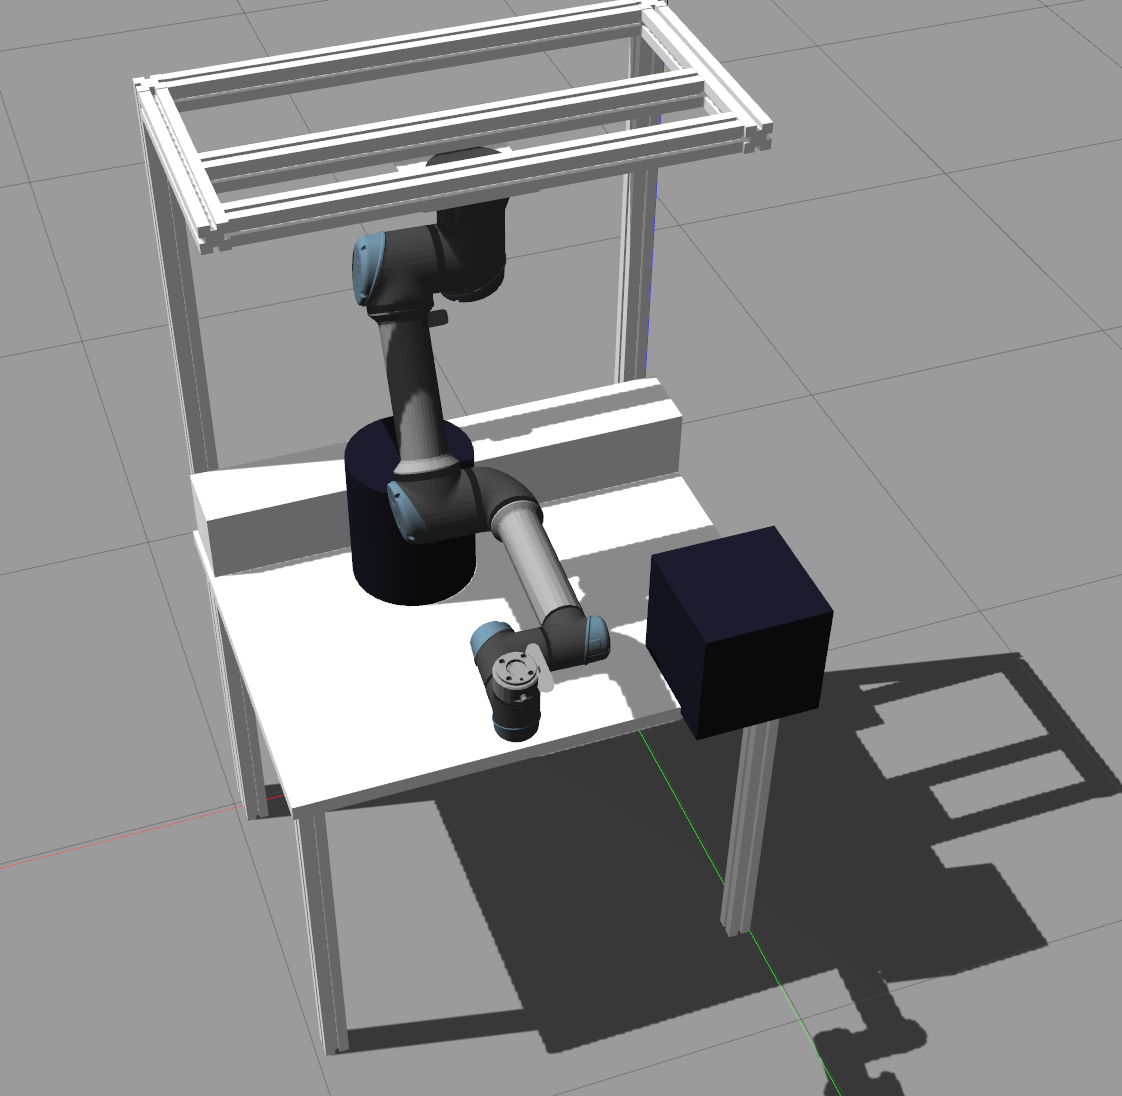
\includegraphics[width=8cm]{pics/workbench.png}
	\caption{Robot workspace with two obstacles (in black).}
	\label{fig:workspace}
\end{figure} 


\begin{table}[h!]
	\caption{Obstacles parameters}
	\begin{center}
		\begin{tabular}{@{} l l l l @{}}
		\hline\hline
			\textbf{Parameter} & {\textbf{Symbol}} &Cylinder    & Cube \\ 
			\hline
			Center [$m$] & $x_c$&  $\mat{0.6 &0.25&1.0}$  & $\mat{0.125 &0.75& 0.975}$  \\
			Height [$m$] & $h_{cyl}$&  0.125  & -    \\
			Radius [$m$]& $R_{cyl}$&  16  & -    \\
			Side [$m$]  & $d_{cube}$& -   & 0.25    \\
		\hline\hline
		\end{tabular}
		\label{tab:obstacles}
	\end{center}
\end{table}
%

Let's compute the repulsive potential field force for each of them from the end-effector $p$:

\begin{equation}
\mathbf{f}_{r, i}(p)=-\nabla_{p} U_{r, i}(p)=\left\{\begin{array}{ll}
\frac{k_{r, i}}{\rho_{i}^{2}(p)}\left(\frac{1}{\rho_{i}(p)}-\frac{1}{d_{0}}\right) \nabla_{p} \rho_{i}(p) & \text { if } \rho_{i}(p) \leq d_{0} \\
0 & \text { if } \rho_{i}(p)>d_{0}
\end{array}\right.
\end{equation}
 
where $\rho$ is the distance $\Vert p - y\Vert$ from the control point $p$ to the closest point $y$ on obstacle $CO_i$, while  $k_{r, i}$ is the field strength and $d_0$ the distance from the obstacle after which the field vanish. Where the derivative $ \nabla_{p} \rho_{i}(p) $ can be approximated to be:

\begin{equation}
 \nabla_{p} \rho_{i}(p) = \frac{ p_k - y}{\Vert p_k -y \Vert}
\end{equation}


 Note that because we have convex obstacles to compute the closest point $y$ on the obstacle we can solve a constrained convex optimization problem:

\begin{align}
y^* &= \argmin_y \Vert p - y \Vert ^2\\
&s.t.  \nonumber  \\
   &Ay \leq b   \nonumber \\ 
   &\Vert Cy + d \Vert \leq f \nonumber 
\end{align}

where $   Ay \leq b$ and $ \Vert Cy + d \Vert \leq f$ are appropriate linear (cube) and second order cone constraints (cylinder)
that  represent the space occupied by the object.
Now, we can exploit the additive property of potential fields to cumulate their influences. 

\begin{align}
\mathbf{f}_{r}(p) = f_a(p) + \mathbf{f}_{r, {cyl}}(p) + \mathbf{f}_{r, {cube}}(p)
\end{align}




Additionally we want to keep also the joints (e.g. not only the end effector) 
away from the obstacles. We can therefore introduce other $p_k$  control 
points, at least one  for each link. 
We discretize the robot using 5 control points: 

\begin{verbatim} 
	'tool0', 
	'upper_arm_link_middle', 
	'forearm_link',  
	'forearm_link_middle', 
	'forearm_link_end'
\end{verbatim}

Add the missing frames:\\
\codeword{'upper_arm_link_middle', 'forearm_link_middle', 'forearm_link_end'} 
to the URDF of the robot and get their position and Jacobians with Pinocchio.
Note that you will have to compute only the repulsive force for these control points as we for the end-effector.

Now we can map these virtual forces into either 
joint torques of set-points for joint velocity, depending on the planning strategy (the latter being more reactive ) 
and sum over the $N$ control points. 
We chose to implement the torque approach  therefore we need to remember 
to add a damping $B$ at the joint level otherwise the system will oscillate forever around the goal:

\begin{equation}
\tau =-\sum_{k=1}^{N-1} \mathbf{J}_{i}^{T}(\mathbf{q}) \nabla_{p} U_{r}\left(\mathbf{p}_{k}\right)-\mathbf{J}_{N}^{T}(\mathbf{q}) \nabla_{p} U_{t}\left(\mathbf{p}_{P}\right)+B \dot{q}
\end{equation}

The signature of the function is given below:
%
\begin{verbatim} 
tau_ffwd = computeTorques (actual_pos, goal):
\end{verbatim}
The input arguments to this function are explained below:
\begin{verbatim} 
actual_pos: An array specifying the coordinates of the actual end-effector location
goal: An array specifying the coordinates of the goal
\end{verbatim}

On every iteration the planner should update the set-point for the  torques of the robot based on the gradient
values computed.  Observe how the end-effector reaches the goal and changes its trajectory to  stay away from  the obstacles. 



%%TODO implement for speed

\end{document}